\documentclass{resume} % Use the custom resume.cls style

\usepackage[left=0.75in,top=0.6in,right=0.75in,bottom=0.6in]{geometry} % Document margins
\usepackage{xcolor}
\usepackage{hyperref}
\hypersetup{
    colorlinks=true,
    linkcolor=blue,
    filecolor=magenta,      
    urlcolor=teal,
}
\usepackage{graphicx}
\newcommand{\tab}[1]{\hspace{.2667\textwidth}\rlap{#1}}
\newcommand{\itab}[1]{\hspace{0em}\rlap{#1}}
\name{Emilio Berti} % Your name
% \address{\centering 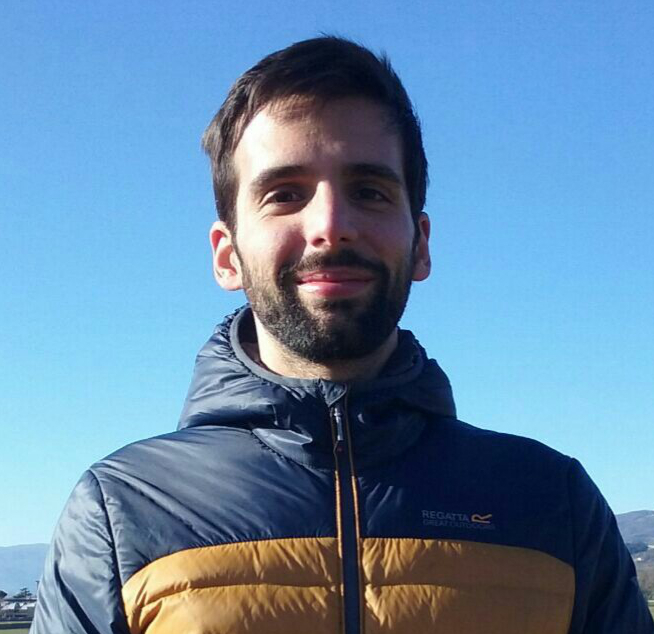
\includegraphics[width=0.30\textwidth]{Emilio.jpg}}
\address{
+49 1525 89 53 261\\ 
emilio.berti.academia@gmail.com \\ 
\href{https://scholar.google.com/citations?user=5KPh-oUAAAAJ&hl=en}{Google scholar} \\
\href{https://orcid.org/0000-0001-9286-011X}{ORCID} \\
\href{https://emilio-berti.github.io/}{website}
}

\begin{document}

\begin{rSection}{Summary}
I am a theoretical ecologist with a passion for math and computing. I have a strong quantitative background,
with expertise in mathematical and statistical modelling of complex systems using big databases at large
spatio-temporal scales. I have worked in many different fields of biology, from molecular muscle physiology
to macroecology and biogeography. I am very open minded to other cultures and societies: I am Italian,
my wife is Bulgarian, we met in Denmark, and we live in Germany. I am an avid reader of ancient history
and I love sumo.

\end{rSection}

\begin{rSection}{Professional experience}

{\bf PostDoctoral researcher} \hfill {\em October 2020 -- Present}\\
Theory in Biodiversity Science, German Centre for Integrative Biodiversity Research (\textsc{iDiv}), Leipzig, Germany.

{\bf Scientific consultant} \hfill {\em May 2020 -- July 2020}\\
Department of Bioscience, Aarhus University, Aarhus, Denmark.

{\bf Teaching assistant} \hfill {\em February 2017 -- April 2020}
\\Department of Biology, Aarhus University, Aarhus, Denmark.

\end{rSection}

\begin{rSection}{Education}
{\bf PhD} \hfill {\em February 2017 -- June 2020} \\
Section of Ecoinformatics and Biodiversity, Department of Biology, Aarhus University, Aarhus, Denmark.

{\bf Visiting PhD student} \hfill {\em Fall 2018} \\
Department of Ecology and Evolution, University of Chicago, Chicago, IL.

{\bf MSc in Biology} \hfill {\em 2013 -- 2016} \\
Department of Ecology and Evolution, University of Florence, Florence, Italy.

{\bf BSc in Biology} \hfill {\em 2009 -- 2012} \\
Department of Physiology, University of Florence, Florence, Italy.
\end{rSection}

\begin{rSection}{Grants}
\begin{tabular}{l l}
{\em 2024} & U. S. National Science Foundation (NSF). Understanding impacts of climatic variability on\\
           & distributions of species. 800,000\$ awarded to Prof. Daniel Reuman (PI), Emilio Berti (co-PI),\\
           & Townsend Peterson (co-PI), and Jorge L. Soberon (co-PI).
\end{tabular}
\end{rSection}

\begin{rSection}{Relevant skills}
I have developed an outstanding mathematical and theoretical set of skills and successfully applied it to
investigate macroecological and biogeographical drivers of biodiversity.

\textbf{Programming languages} – R, python, bash, C/C++, Stan, javascript (mostly for Google Earth Engine), SQL (postgis flavor).\\
\textbf{Software} – Linux/GNU, Anaconda, RShiny, Google Earth Engine, High-performance computing (HPC, Slurm flavor), Tidyverse, Git, GitHub, Jupyter Notebooks, \LaTeX.\\
\textbf{Methods} – Mathematical modeling, Geographic information systems (GIS), Geoinformatics, Geomatics, Remote sensing, Biostatistics, Data science, Climate analyses, Species distribution modeling, Environmental niche modeling, Machine learning, Bayesian statistics, Ordination and classification, Network theory,
Community assembly, Optimization, Automation.\\
\textbf{Languages} – Italian (native), English (fluent), German (A1 $\rightarrow$ A2.1).
\end{rSection}

\begin{rSection}{Software}
GHCNr: Download and process daily weather data from the Global Historical Climatology Network (GHCN) database. Author, maintainer. \url{https://cran.r-project.org/packages=GHCNr}.\\
enerscape: Compute Energy Landscapes (CRAN). Author, maintainer. \url{https://cran.r-project.org/package=enerscape}.\\
ATNr: Run Allometric Trophic Networks Models (CRAN). Author. \url{https://cran.r-project.org/package=ATNr}.\\
squirrygis: Fast C++ routines to process climate layers (GitHub). Author, maintainer. \url{https://github.com/emilio-berti/squirrygis}.
assembly: Simulate community assembly (GitHub). Author, maintainer. \url{https://github.com/emilio-berti/assembly}.
\end{rSection}

\begin{rSection}{Selected publications}
A full list of my publications can be found at \href{https://scholar.google.com/citations?hl=en&user=5KPh-oUAAAAJ&view_op=list_works&sortby=pubdate}{Google Scholar}.

\begin{enumerate}
    \setlength\itemsep{-0.5em}
    \item \textbf{Berti, E.}, Rosenbaum, B., \& Vollrath Fritz. (2025). Energy landscapes direct the movement preferences of elephants. \textit{Journal of Animal Ecology} (Accepted). 
    \item Li, J., Brose, U., Rosenbaum, B., Ryser, R., \& \textbf{Berti, E}. (2024). Decoding Information Flow and Sensory Pollution: A Systematic Framework for Understanding Species Interactions. \textit{Ecology Letters}. DOI: \href{https://doi.org/10.1111/ele.14522}{10.1111/ele.14522}.
    \item Antunes, A. C., \textbf{Berti, E.}, \dots, \& Gauzens, B. (2024). Linking biodiversity, ecosystem function, and Nature’s contributions to people: a macroecological energy flux perspective. \textit{Trends in Ecology \& Evolution}. DOI: \href{https://doi.org/10.1016/j.tree.2024.01.004}{10.1016/j.tree.2024.01.004}.
    \item Gauzens, B., Brose, U., Delmas, E., \& \textbf{Berti, E}. (2023). ATNr: Allometric Trophic Network models in R. Methods in Ecology and Evolution.
    \item Bauer, B., \textbf{Berti, E.}, ... \& Brose, U. (2022). Biotic filtering by species’ interactions constrains food-web variability across spatial and abiotic gradients. \textit{Ecology letters}. DOI: \href{https://doi.org/10.1111/ele.13995}{10.1111/ele.13995}. (\texttt{Shared first authorship}).
    \item Grenié, M, \textbf{Berti, E.}, ... \& Marten, W. (2022). Harmonizing taxon names in biodiversity data: a review of tools, databases, and best practices. \textit{Methods in Ecology and Evolution}. DOI: \href{https://doi.org/10.1111/2041-210X.13802}{10.1111/2041-210X.13802}.
    \item \textbf{Berti, E.}, Davoli, M., ... \& Vollrath, F. (2021). The r package enerscape: A general energy landscape framework for terrestrial movement ecology. \textit{Methods in Ecology and Evolution}. DOI: \href{https://doi.org/10.1111/2041-210X.13734}{10.1111/2041-210X.13734}.
    \item \textbf{Berti, E.}, Monsarrat, S., Munk, M., Jarvie, S. \& Svenning, J.C. (2020). Body size is a good proxy for vertebrate charisma. \textit{Biological Conservation}. DOI: \href{https://doi.org/10.1016/j.biocon.2020.108790}{10.1016/j.biocon.2020.108790}.
    \item \textbf{Berti, E.} \& Svenning, J.C. (2020). Megafauna extinctions have reduced biotic connectivity worldwide. \textit{Global Ecology and Biogeography}. DOI: \href{https://doi.org/10.1111/geb.13182}{10.1111/geb.13182}.
\end{enumerate}
\end{rSection}

\begin{rSection}{Conference talks as presenter}
\begin{enumerate}
    \setlength\itemsep{-0.5em}
    \item \textbf{Berti, E.}, Rosenbaum, B., Brose, U., \& Vollrath, F. (2023). Energy landscapes direct the movement preferences of elephants. \textit{British Ecological Society annual meeting, Belfast, UK}/
    \item Bauer, B., \textbf{Berti, E.}, \dots, \& Brose, U. (2022). From regional to local scale: biotic interactions shape multilayer food-webs. \textit{SFE-GFO-EEF biannual meeting, Metz, France} (\underline{invited talk}).
    \item \textbf{Berti, E.}, \& Svenning, J.C. (2022). State-space models show that functional replacements of extinct megafauna have distinct habitat preference in a European rewilding area. \textit{SFE-GFO-EEF biannual meeting, Metz, France}.
    \item Grenié, M., \textbf{Berti, E.}, Carvajal-Quintero, J., Winter, M., \& Sagouis (2021). Matching Species Names Across Biodiversity Databases: Sources, tools, pitfalls and best practices for taxonomic harmonization. \textit{TDWG annual meeting, online}.
    \item \textbf{Berti, E.} \& Svenning, J.C. (2019). Megalinkers extinction and the decrease of ecosystem connectivity. \textit{ESA annual meeting, Louisville, KY}.
    \item \textbf{Berti, E.}, Jarvie, S. W., \& Svenning, J.C. (2018). Rewiring food webs via trophic rewilding. \textit{BES annual meeting, Belfast, UK}.
\end{enumerate}
\end{rSection}

\begin{rSection}{Peer review}
As of July 2022, I have reviewed 7 papers for: Ecography (1), Ecology Letters (2), Ecology (1), GigaScience (1), Method in Ecology and Evolution (1), and Scientia Agricola (1). You can find more at my \href{https://publons.com/wos-op/researcher/4208953/emilio-berti/}{Publons profile}.
\end{rSection}

\begin{rSection}{Supervision, mentoring, and teaching}
I am formally co-supervising the PhD candidate Jingyi Li, who is developing a novel mathematical approach for functional responses based on information theory. 
In addition, I provide theoretical, computational, and statistical advice to several members of the TiBS working group at iDiv as well as individual mentoring for PhD students, advising especially on transferable skills and alternative career paths outside academia.
During my PhD, I taught one course per semester, as part of my salary was paid by Aarhus University on the basis of teaching.
In addition, I have regularly organized workshops to teach reproducible research and open data principles and have organized a weekly journal club during my PhD and currently during my PostDoc.
\begin{itemize}
    \setlength\itemsep{-0.5em}
    \item Meta-analyses for Biodiversity (2024 \& 2021) – Teaching assistant (MSc course).
    \item Theoretical Population Ecology (2023) – Teaching assistant (MSc course).
    \item Introduction to scientific programming and tidyverse (2022) (slides) – Lecturer (PhD course).
    \item Introduction to git and GitHub for a fool-proof programming (2022) (course) – Lecturer (PhD course).
    \item Statistical and Geospatial Modelling (2019) – Teaching assistant (MSc course).
    \item Behavioural Biology (2018, 2019) – Teaching assistant (BSc course).
    \item Geographic Information System (2017) – Lab assistant (BSc course).
    \item Cleaning online repository data for use in biogeography and macroecology (2019) -- Co-organizer (workshop).
    \item Running a species distribution model in R (2019) -- Co-organizer (workshop).
    \item A (very) gentle introduction to Linux (2019) -- Organizer (workshop).
\end{itemize}
\end{rSection}

\begin{rSection}{Collaborations}
I have moved several times to pursue my career dreams and, being a friendly person, I established personal and professional ties with the people I met. My network of current collaborators include:
\begin{itemize}
    \setlength\itemsep{-0.5em}
    \item Prof. Jens-Christian Svenning, Aarhus University, Aarhus, Denmark.
    \item Prof. Ulrich Brose, Jena University, Jena, Germany.
    \item Prof. Daniel Reuman, Kansas University, Lawrence, KS, USA.
    \item Prof. Giacomo Santini, Universit\`{a} degli Studi di Firenze, Florence, Italy.
    \item Prof. Kai Yue, Fujian Normal University, Fuzhou, China.
    \item Prof. Neil Carter, University of Michigan, Ann Arbor, MI, USA.
    \item Prof. Fritz Vollrath, University of Oxford, Oxford, UK.
\end{itemize}
\end{rSection}

\end{document}
